As we can see in the use cases discussed in the previous section, it can be hard
to say if the use of flash loans is malicious. As mentioned, flash loans do not
enable new things, it merely allows everyone to trade with large amounts of
capital (within a single transaction), as opposed to only the ones with a lot of
liquidity. We would consider a use case like arbitrage as benign. While you
\textit{do} make money on market instabilities, you stabilize the market by
doing so. For example, Uniswap version 2 depends on arbitrage to maintain a
``correct'' exchange rate, so here flash loans just enables everyone to join in.
Where use cases such as wash trading (and oracle manipulation as we will see in
section \ref{ex}) are clearly malicious, since these practices distort the
market to gain a profitable opportunity without adding anything to the market.
Then finally we have collateral swapping, and liquidation auctions, which are
seems like a benign, or maybe even good use.\\
\begin{wrapfigure}[20]{r}{7cm}
  \centering
  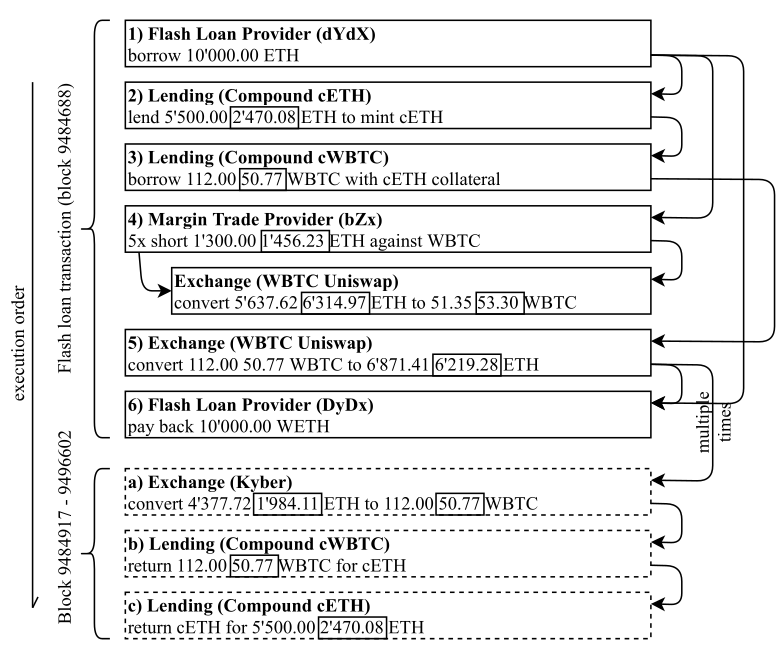
\includegraphics[width=8cm]{assests/pump-and-arb}
  \caption{This figure illustrates the pump and arbitrage
    procedure. Note that the numbers in boxes (along with the 50.77
    WBTC in step 5) should be ignored as these are not used in this
    report \cite[p. 5 fig. 6]{attack}}
  \label{fig:pumpAndArb}
\end{wrapfigure}
\begin{wrapfigure}[20]{r}{7cm}
  \centering
  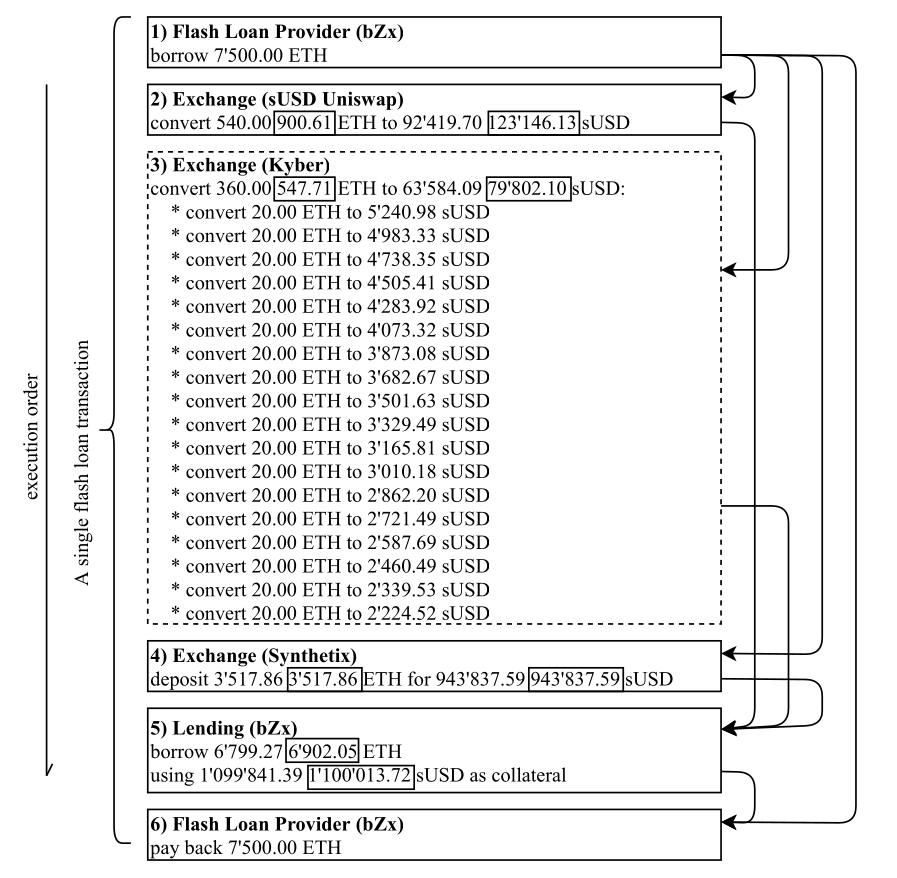
\includegraphics[width=8cm]{assests/oracle}
  \caption{This figure illustrates the oracle manipulation
    procedure. Note that the numbers in boxes should be ignored as
    these are not used in this report \cite[p. 6 fig. 7]{attack}}
  \label{fig:oracle}
\end{wrapfigure}
So flash loans are not inherently good or bad, but they enable both kinds of
behaviors. They are possible because of the discrete nature of the blockchain,
as opposed to the continuous nature of traditional finance.
